%%%%%%%%%%%%%%%%%%%%%%
%
%   Work related to the verification of the datasets
%
%%%%%%%%%%%%%%%%%%%%%%

\section{Slices of Datacubes}

\section{Power spectra from Theory}

\TODO{Provide some camb and class power spectra here. }

\section{Powerspectra from Simulations}
\begin{figure}
    \centering
    % 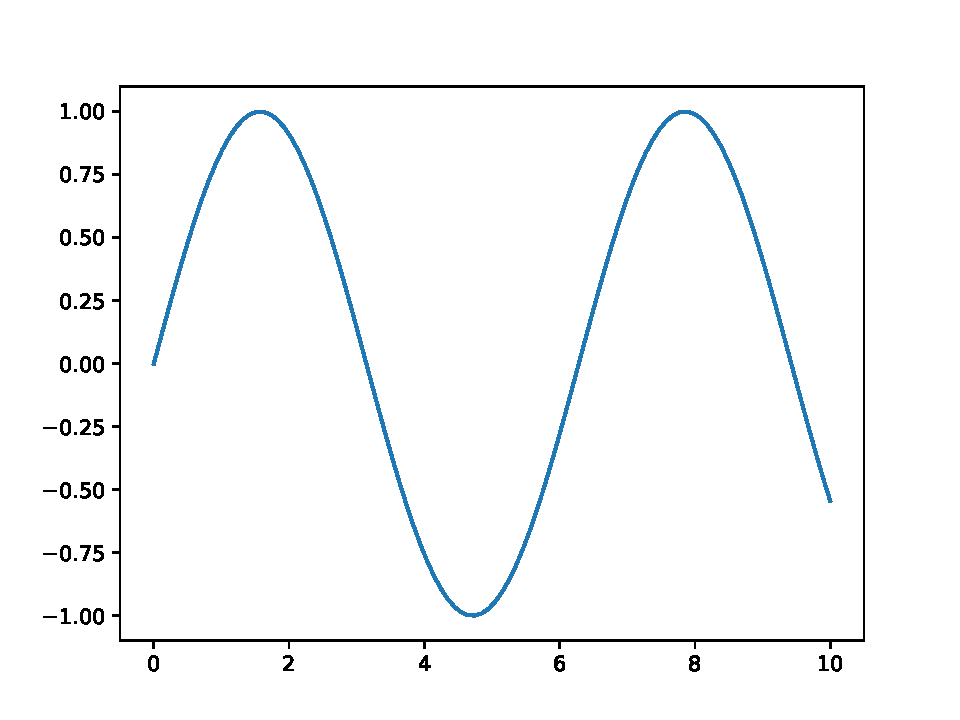
\includegraphics[width=\linewidth]{main/test.pdf}
    \includeimage[width=\linewidth]{nine_matter_power_spectra}
  \end{figure}

  \begin{figure}
    \centering
    % 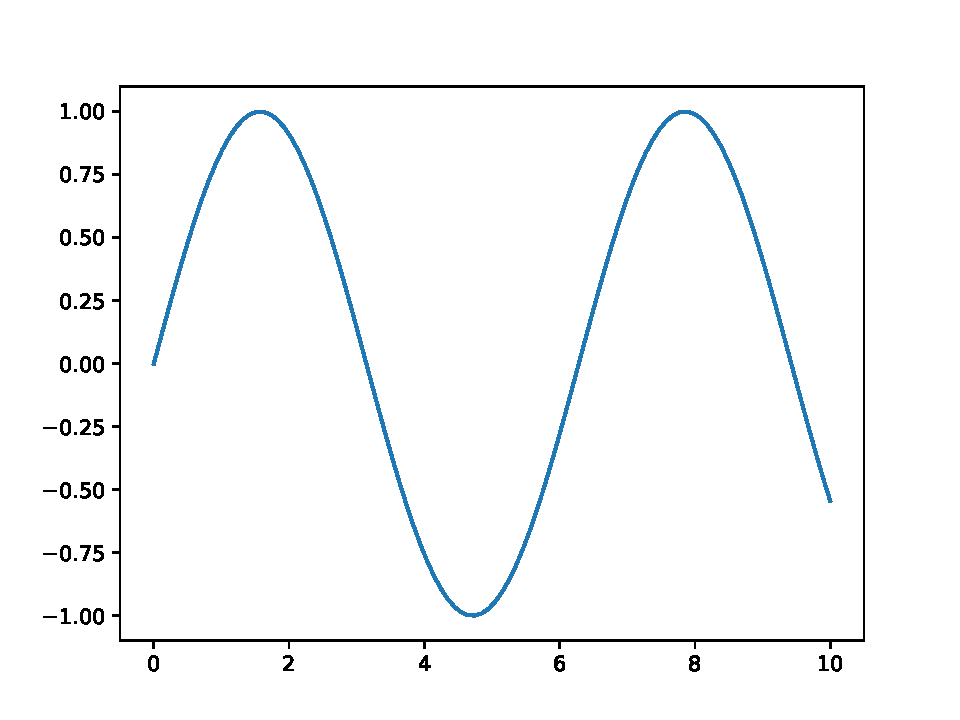
\includegraphics[width=\linewidth]{main/test.pdf}
    \includeimage[width=\linewidth]{average_matter_power_spectrum}
  \end{figure}

\section{Powerspectra from Datacubes}

\section{Analytical Bispectra}

\begin{equation}
  B^{(3)}(k_1,k_2,k_3) = 2\mathcal{P}(k_1)\mathcal{P}(k_2)F_2(\vec{k}_1, \vec{k}_2) + \mathrm{cyc}
\end{equation}

\begin{equation}
  F_2(\vec{k}_1,\vec{k}_2) = \frac{5}{7} + \frac{x}{2}\left(\frac{k_1}{k_2}+\frac{k_2}{k_1}\right) + \frac{2}{7}x^2,
\end{equation}
where $x = \hat{\vec{k}}_1 \cdot \hat{\vec{k}}_2 = \cos{\theta_{12}}$, where $\theta_{12}$ is the angle spanned by $\vec{k}_1$ and $\vec{k}_2$. We could thus consequently write: $F_2(\vec{k}_1,\vec{k_2}) = F_2(k_1,k_2,\theta_{12})$

Given $k_1$ and $k_2$ and $\theta_{12}$ we have the following relations \TODO{Include figure here}:

\begin{equation}
  \begin{split}
    \alpha &= \pi-\theta_{12}\\
    \beta &= \pi-\theta_{23}\\
    \gamma &= \pi-\theta_{31}
  \end{split}
\end{equation}

From cosine rule:
\begin{equation}
  k_3 = \sqrt{k_1^2 + k_2^2 - 2k_1k_2\cos\alpha}
\end{equation}

From the rule of sines \TODO{explain more?}:
\begin{equation}
  \begin{split}
    \beta &= \arcsin\left(\frac{k_1}{k_3}\sin\alpha\right)\\
    \gamma &= \arcsin\left(\frac{k_2}{k_3}\sin\alpha\right)
  \end{split}
\end{equation}


\section{Bispectra from Cube}

